
%(BEGIN_QUESTION)
% Copyright 2006, Tony R. Kuphaldt, released under the Creative Commons Attribution License (v 1.0)
% This means you may do almost anything with this work of mine, so long as you give me proper credit

En \textit{strain gauge} (tøyningsmåler) er en enhet som brukes til å måle tøyning (kompresjon eller utvidelse) i et fast materiale ved å lage en motstandsforandring proporsjonal med tøyningen.  Når måleren deformeres, endres den elektriske motstanden litt:

$$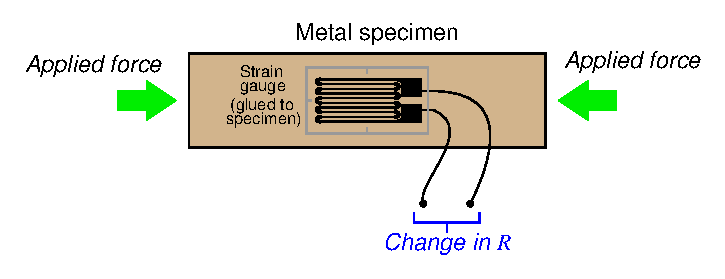
\includegraphics[width=15.5cm]{i00181x02.eps}$$

Forklar \textit{hvorfor} den elektriske motstanden i en strain gauge endres når den strekkes og krymper, og knytt også retningen på motstandsforandringen (mer eller mindre) til retningen på påført kraft.

\vskip 10pt

Følgende strain gauge er vist koblet i en ``quarter-bridge''-krets (det vil si at bare en fjerdedel av broen måler tøyning aktivt, mens de tre andre fjerdedelene har fast motstand):

$$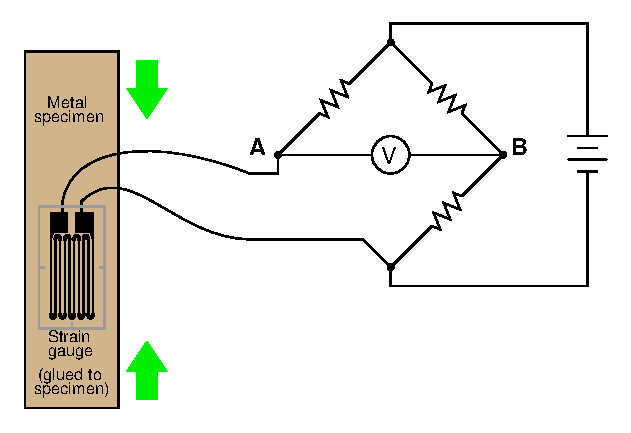
\includegraphics[width=15.5cm]{i00181x01.eps}$$

Forklar hva som ville skjedd med spenningen målt over denne brokretsen ($V_{AB}$) hvis strain gaugen ble \textit{komprimert}, forutsatt at broen starter i balanse uten tøyning i måleren.

\vskip 20pt \vbox{\hrule \hbox{\strut \vrule{} {\bf Suggestions for Socratic discussion} \vrule} \hrule}

\begin{itemize}
\item{} En god problemløsningsteknikk ved analyse av endringsretninger i en Wheatstone-bro er å se på \textit{grensetilfeller}.  I stedet for å spørre hva som skjer hvis strain gauge-motstanden endres litt, spør vi hva som skjer hvis motstanden endres \textit{drastisk} (f.eks. helt åpen eller helt kortsluttet).  Forklar hvordan vi kan bruke denne teknikken på denne kretsen.
\item{} Strain gauges brukes mye i bil- og luftfartsindustri for å studere mekanisk tøyning i konstruksjoner.  Forklar hvordan en strain gauge kan brukes til å måle tøyning i noe som en lastebilaksel.
\end{itemize}

\underbar{file i00181}
%(END_QUESTION)





%(BEGIN_ANSWER)

Når en strain gauge strekkes, blir lederne lengre og tynnere, og motstanden øker.  Når en strain gauge komprimeres, blir lederne kortere og tykkere, og motstanden minker.  Brokretsen blir mer ubalansert når strain gauge-motstanden endres fra nøytralverdien.

\vskip 10pt

I denne kretsen minker spenningsfallet over strain gaugen når den komprimeres.  Dette gjør potensialet i punkt A mer negativt, slik at $V_{AB}$ utvikles med A negativ og B positiv.


%(END_ANSWER)





%(BEGIN_NOTES)






\vfil \eject

\noindent
{\bf Prep Quiz:}

A \textit{strain gauge}:

\begin{itemize}
\item{} Measures applied force by changing its electrical resistance accordingly
\vskip 5pt 
\item{} Measures vibration by creating an AC voltage when shaken or accelerated
\vskip 5pt 
\item{} Indicates applied force with a dial-style face like a gauge or bathroom scale
\vskip 5pt 
\item{} Stabilizes voltage in a DC ``Wheatstone bridge'' circuit for high accuracy
\vskip 5pt 
\item{} Acts as a thermometer, sensing metal fatigue caused by temperature
\vskip 5pt 
\item{} Measures electrical resistance by changing length according to how hot it is
\end{itemize}

%INDEX% Measurement, strain gauge

%(END_NOTES)

